\documentclass{beamer}
\usepackage{graphicx}
\usepackage{tikz}
\usetikzlibrary{shapes,arrows}
\usepackage{tikz}
\usepackage{amsfonts}
\usepackage{amssymb}
\usetheme{default}
%\usecolortheme{seahorse}
\usepackage{default}
  \setbeamertemplate{footline}[page number]
\usepackage{multirow}
\setbeamertemplate{navigation symbols}{}
\setbeamertemplate{frametitle}[default][center]
\setbeamerfont{frametitle}{shape=\scshape}

\usepackage{xcolor}

\usepackage[flushleft]{threeparttable}

{\title{\textsc{Numerical Methods Lecture XIV: \\ Simulated Estimation} \\ \tiny (See Keane and Moffitt 1996)}
\author{Trevor Gallen}
\date{}
\begin{document}
\renewcommand*{\inserttotalframenumber}{\pageref{lastframe}}

\begin{frame}
\titlepage
\end{frame}

%\begin{frame}
%\frametitle[alignment=center]{Agenda}
%\begin{itemize}
%\item Homework 1 up, homework 2 turned in up.
%\bigskip
%\item Patrick Bayer Thursday
%\bigskip
%\item Matt Notowidigdo Friday \uncover<2->{\textcolor{red}{(!)}}
%\bigskip
%\item Today:
%\bigskip
%\begin{itemize}
%\item Cook
%\bigskip
%\item Brief GMM \& Estimation
%\end{itemize}
%\end{itemize}
%\end{frame}

%\begin{frame}
%\frametitle[alignment=center]{First, an aside from last class...}
%\begin{itemize}
%\item We frequently see GMM written down as something like:
%$$E(f(x_t,\beta_0)=0$$
%\item Where $f$ has $r$ coordinates and $\beta_0$ is an unknown vector in parameter space %$\mathbb{P}\subset\mathbb{R}^k$
%\item<2-> Identification comes from:
%$$E(f(x_t,\beta))=0\iff \beta=\beta_0$$
%\item<3-> We set our sample calculation as a function of $\beta$:
%$$g_N(\beta)=\frac{1}{N}\sum_{t=1}^Nf(x_t,\beta)$$
%\item<3-> And choose $\beta$ to minimize the quadratic form:
%$$b_N=\arg\underset{\beta\in\mathbb{P}}{\min} g_N(\beta)'Wg_N(\beta)$$
%\end{itemize}
%\end{frame}

%\begin{frame}
%\frametitle[alignment=center]{Understanding GMM-I}
%\begin{itemize}
%\item We frequently see GMM written down as something like:
%$$E(f(x_t,\beta_0)=0$$
%\item Where $f$ has $r$ coordinates and $\beta_0$ is an unknown vector in parameter space $\mathbb{P}\subset\mathbb{R}^k$
%\item<2-> Identification comes from:
%$$E(f(x_t,\beta))=0\iff \beta=\beta_0$$
%\item<3-> We set our sample calculation as a function of $\beta$:
%$$g_N(\beta)=\frac{1}{N}\sum_{t=1}^Nf(x_t,\beta)$$
%\item<3-> And choose $\beta$ to minimize the quadratic form:
%$$b_N=\arg\underset{\beta\in\mathbb{P}}{\min} g_N(\beta)'Wg_N(\beta)$$
%\end{itemize}
%\end{frame}

%\begin{frame}
%\frametitle[alignment=center]{Understanding GMM-II}
%$$b_N=\arg\underset{\beta\in\mathbb{P}}{\min} g_N(\beta)'Wg_N(\beta)$$
%\begin{itemize}
%\item This should look familiar!
%\bigskip
%\item<1-> Think of $g_N(\beta)$ as your error: it should be zero.
%\bigskip
%\item<2-> Then this looks like:
%$$b_N=\arg\underset{\beta\in\mathbb{P}}{\min} \sum_{i=1}^Nw_i\epsilon_i^2$$
%\item<3-> Like weighted least squares
%\end{itemize}
%\end{frame}

%\begin{frame}
%\frametitle[alignment=center]{Understanding Structural Estimation - I}
%\begin{itemize}
%\item We frequently have some model with data $y_i$ and $x_i$, and unknown parameters $%\beta$:
%$$y_i=x_i\beta$$
%\item Then we have the moment condition:
%$$E(y_i-x_i\beta)=0$$
%\item Letting $z_i=\{x_i,y_i\}$, then we could write this as:
%$$f(z,\beta)=(y_i-x_i\beta)$$
%\item With the property:
%$$E(f(z,\beta))=0$$
%\item Which is in the same form as what we wrote as a moment condition above:
%$$E(f(x_t,\beta))=0$$
%\item Linear regressions are a special case of structural estimation
%\end{itemize}
%\end{frame}

%\begin{frame}
%\frametitle[alignment=center]{Understanding Structural Estimation - II}
%\begin{itemize}
%\item Why might they seem so different?
%\bigskip
%\item The vector of stacked $f(x_t,\beta)$'s is pretty simple for linear estimation:
%$$\left[\begin{array}{c}E(y_1-x_1\beta) \\ E(y_2-x_2\beta) \\ \vdots \\ E(y_N-x_N\beta)\end{array}\right]=\left[\begin{array}{c}0 \\ 0 \\ \vdots \\ 0\end{array}\right]$$
%\item The stacked $f$'s might be completely different for structural models
%$$\left[\begin{array}{c}E(y_1-x_1\beta_1) \\ E(x_1x_2-\beta_2) \\ \vdots \\ E(y_1+y_2 - \beta_1^{\beta_2})\end{array}\right]=\left[\begin{array}{c}0 \\ 0 \\ \vdots \\ 0\end{array}\right]$$
%\item Is this offensive?
%\end{itemize}
%\end{frame}

\begin{frame}
\frametitle[alignment=center]{Statutory Marginal Tax Rates-1}
\begin{figure}
\centering
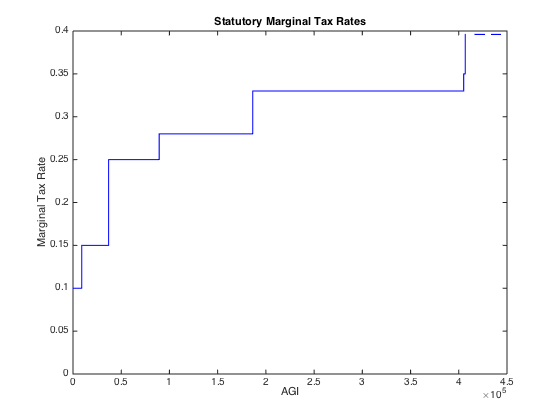
\includegraphics[scale=0.5]{STR_1}
\end{figure}
\end{frame}


\begin{frame}
\frametitle[alignment=center]{Implicit Marginal Tax Rates-1}
\begin{figure}
\centering
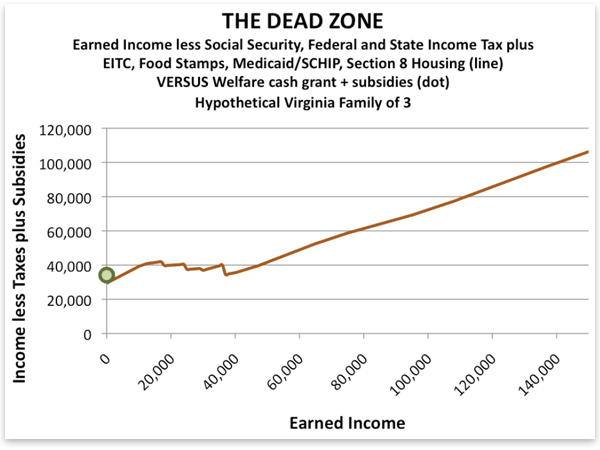
\includegraphics[scale=0.5]{ITR_1}
\end{figure}
\end{frame}

\begin{frame}
\frametitle[alignment=center]{Implicit Marginal Tax Rates-2}
\begin{figure}
\centering
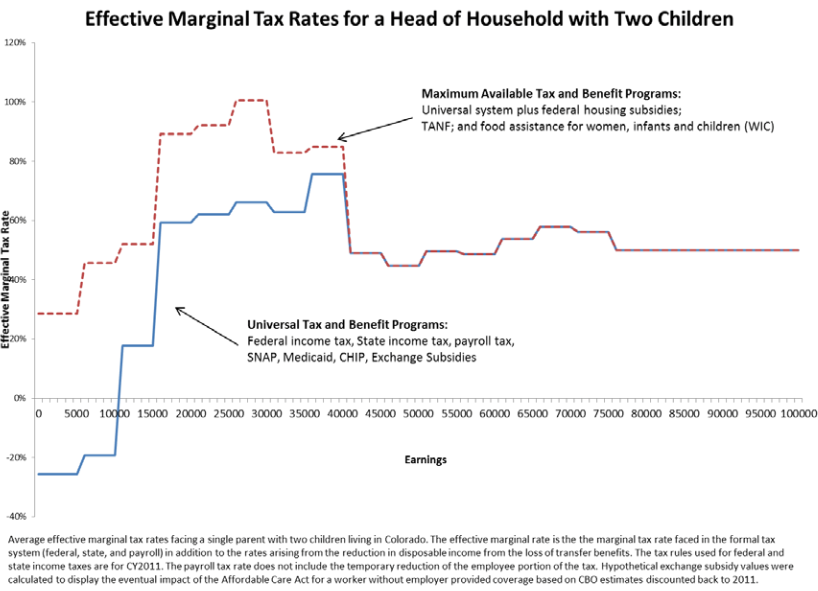
\includegraphics[scale=0.35]{ITR_2}
\end{figure}
\end{frame}

\begin{frame}
\frametitle[alignment=center]{Implicit Marginal Tax Rates-3}
\begin{figure}
\centering
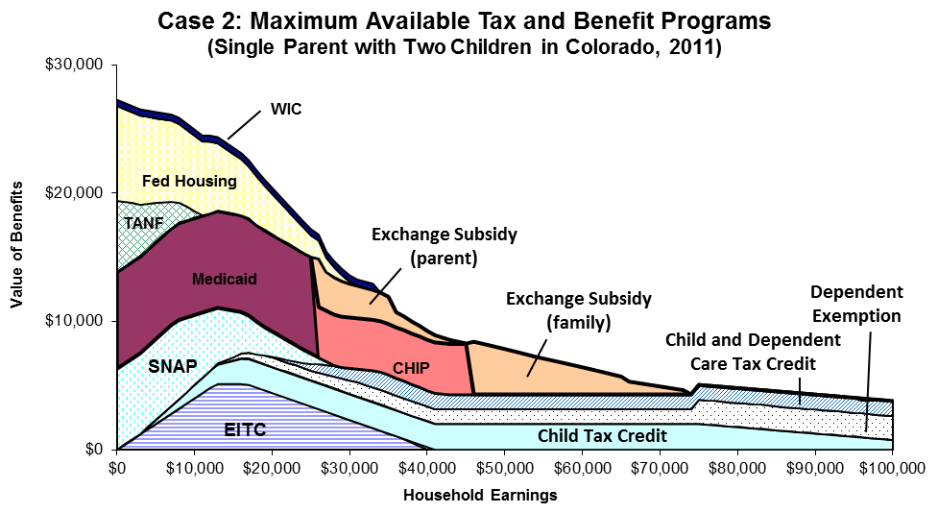
\includegraphics[scale=0.35]{ITR_3}
\end{figure}
\end{frame}

\begin{frame}
\frametitle[alignment=center]{The problem is complicated!}
\begin{itemize}
\item We spend trillions on transfer programs
\bigskip
\item Implicit marginal tax rates frequently bigger deal than statutory tax rates
\bigskip
\item Now, if you're on one program you're on a lot of them
\bigskip
\item In Keane and Moffitt (circa 1989)
\begin{itemize}
\item  89\% of AFDC recipients were on Medicaid and Food Stamps
\item 42\% of AFDC recipients were on some fourth program (like housing)
\end{itemize} 
\item Enormous implicit marginal tax rates interact
\end{itemize}
\end{frame}

\begin{frame}
\frametitle[alignment=center]{Keane \& Moffitt}
\begin{itemize}
\item Look at female heads
\bigskip
\item AFDC, Food stamps, housing, and labor supply
\bigskip
\item Produce four-equation model
\bigskip
\item Simulate outcomes given parameters
\bigskip
\item Estimate parameters
\end{itemize}
\end{frame}

\begin{frame}
\frametitle[alignment=center]{Illustrative Cumulative Tax Rates: CA}
\begin{table}
\centering
\begin{tabular}{p{2cm}p{1.3cm}p{1.3cm}p{1.3cm}p{1.5cm}p{1.5cm}}
 &  \multicolumn{3}{c}{Weekly Income} & \multirow{3}{*}{\parbox{1.5cm}{Tax Rate from H=0 to H=20}} & \multirow{3}{*}{\parbox{1.5cm}{Tax Rate from H=20 to H=40}} \\
 \cline{2-4}
  &  \multirow{3}{*}{$H=0$} & \multirow{3}{*}{$H=20$} & \multirow{3}{*}{$H=40$} & &  \\
  & & & & \\
    & & & & \\
\hline
\underline{California} &  &  &  &  &  \\
Earnings & 0 & 104 & 208 & $\cdot$ & $\cdot$\\ 
AFDC & 124 & 30 & 0 & $0.90$ & $0.29$\\ 
Food Stamp & 16 & 16 & 0 & $0$ & $0.15$\\ 
Housing  & 138 & 132 & 107 & $0.06$ & $0.24$\\ 
Taxes & 0 & -8 & -26 & $0.08$ & $0.17$\\ 
Work Expns. & 0 & -21 & -21 & $0.20$ & $0$\\ 
Net Income & 278 & 253 & 268 & $\cdot$ & $\cdot$\\ 
\multirow{2}{*}{\parbox{2cm}{Cumulative Tax Rate}} & \multirow{2}{*}{$\cdot$} & \multirow{2}{*}{$\cdot$} & \multirow{2}{*}{$\cdot$} & \multirow{2}{*}{$1.24$} & \multirow{2}{*}{$0.86$}\\
\end{tabular}
\end{table}
\end{frame}

\begin{frame}
\frametitle[alignment=center]{Illustrative Cumulative Tax Rates: MN}
\begin{table}
\centering
\begin{tabular}{p{2cm}p{1.3cm}p{1.3cm}p{1.3cm}p{1.5cm}p{1.5cm}}
 &  \multicolumn{3}{c}{Weekly Income} & \multirow{3}{*}{\parbox{1.5cm}{Tax Rate from H=0 to H=20}} & \multirow{3}{*}{\parbox{1.5cm}{Tax Rate from H=20 to H=40}} \\
 \cline{2-4}
  &  \multirow{3}{*}{$H=0$} & \multirow{3}{*}{$H=20$} & \multirow{3}{*}{$H=40$} & &  \\
  & & & & \\
    & & & & \\
\hline
\underline{Minnesota} &  &  &  &  &  \\
Earnings & 0 & 104 & 208 & $\cdot$ & $\cdot$\\ 
AFDC & 117 & 25 & 0 & $0.88$ & $0.24$\\ 
Food Stamp & 19 & 19 & 0 & $0$ & $0.18$\\ 
Housing  & 97 & 91 & 64 & $0.06$ & $0.26$\\ 
Taxes & 0 & -8 & -26 & $0.08$ & $0.17$\\ 
Work Expns. & 0 & -21 & -21 & $0.20$ & $0$\\ 
Net Income & 233 & 210 & 225 & $\cdot$ & $\cdot$\\ 
\multirow{2}{*}{\parbox{2cm}{Cumulative Tax Rate}} & \multirow{2}{*}{$\cdot$} & \multirow{2}{*}{$\cdot$} & \multirow{2}{*}{$\cdot$} & \multirow{2}{*}{$1.22$} & \multirow{2}{*}{$0.86$}\\
\end{tabular}
\end{table}
\end{frame}
\begin{frame}
\frametitle[alignment=center]{Illustrative Cumulative Tax Rates: OH}
\begin{table}
\centering
\begin{tabular}{p{2cm}p{1.3cm}p{1.3cm}p{1.3cm}p{1.5cm}p{1.5cm}}
 &  \multicolumn{3}{c}{Weekly Income} & \multirow{3}{*}{\parbox{1.5cm}{Tax Rate from H=0 to H=20}} & \multirow{3}{*}{\parbox{1.5cm}{Tax Rate from H=20 to H=40}} \\
 \cline{2-4}
  &  \multirow{3}{*}{$H=0$} & \multirow{3}{*}{$H=20$} & \multirow{3}{*}{$H=40$} & &  \\
  & & & & \\
    & & & & \\
\hline
\underline{Ohio} &  &  &  &  &  \\
Earnings & 0 & 104 & 208 & $\cdot$ & $\cdot$\\ 
AFDC & 60 & 0 & 0 & $0.58$ & $0$\\ 
Food Stamp & 44 & 30 & 4 & $0.13$ & $0.29$\\ 
Housing  & 87 & 71 & 37 & $0.15$ & $0.33$\\ 
Taxes & 0 & -8 & -26 & $0.08$ & $0.17$\\ 
Work Expns. & 0 & -21 & -21 & $0.20$ & $0$\\ 
Net Income & 191 & 176 & 202 & $\cdot$ & $\cdot$\\ 
\multirow{2}{*}{\parbox{2cm}{Cumulative Tax Rate}} & \multirow{2}{*}{$\cdot$} & \multirow{2}{*}{$\cdot$} & \multirow{2}{*}{$\cdot$} & \multirow{2}{*}{$1.14$} & \multirow{2}{*}{$0.75$}\\
\end{tabular}
\end{table}
\end{frame}

\begin{frame}
\frametitle[alignment=center]{Illustrative Cumulative Tax Rates: KS}
\begin{table}
\centering
\begin{tabular}{p{2cm}p{1.3cm}p{1.3cm}p{1.3cm}p{1.5cm}p{1.5cm}}
 &  \multicolumn{3}{c}{Weekly Income} & \multirow{3}{*}{\parbox{1.5cm}{Tax Rate from H=0 to H=20}} & \multirow{3}{*}{\parbox{1.5cm}{Tax Rate from H=20 to H=40}} \\
 \cline{2-4}
  &  \multirow{3}{*}{$H=0$} & \multirow{3}{*}{$H=20$} & \multirow{3}{*}{$H=40$} & &  \\
  & & & & \\
    & & & & \\
\hline
\underline{Kansas} &  &  &  &  &  \\
Earnings & 0 & 104 & 208 & $\cdot$ & $\cdot$\\ 
AFDC & 76 & 0 & 0 & $0.73$ & $0$\\ 
Food Stamp & 38 & 31 & 0 & $0.07$ & $0.30$\\ 
Housing  & 68 & 64 & 31 & $0.04$ & $0.32$\\ 
Taxes & 0 & -8 & -26 & $0.08$ & $0.17$\\ 
Work Expns. & 0 & -21 & -21 & $0.20$ & $0$\\ 
Net Income & 82 & 170 & 192 & $\cdot$ & $\cdot$\\ 
\multirow{2}{*}{\parbox{2cm}{Cumulative Tax Rate}} & \multirow{2}{*}{$\cdot$} & \multirow{2}{*}{$\cdot$} & \multirow{2}{*}{$\cdot$} & \multirow{2}{*}{$1.12$} & \multirow{2}{*}{$0.79$}\\
\end{tabular}
\end{table}
\end{frame}

\begin{frame}
\frametitle[alignment=center]{Keane \& Moffitt: Utility}
\begin{itemize}
\item $U$ is:
$$U(H,Y,P_1,P_2,P_3)=\overline{U(H,Y)}-\psi_1P_1-\psi_2P_2-\psi_3P_3$$
\item Where $H$ is hours of work.
\bigskip
\item Y is disposable income.
\bigskip
\item $P_j$ is a dummy variable for participation in program $j$.
\bigskip
\item $\psi_j$ is the marginal disutility of participating in program $j$.
\bigskip
\item Limit $H\in\{0,20,40\}$.  Limits to $3\cdot2^3=24$ possibilities.
\end{itemize}
\end{frame}


\begin{frame}
\frametitle[alignment=center]{Keane \& Moffitt: Budget Constraint}
\begin{itemize}
\item Disposable income is defined as:
$$Y(H,P_1,P_2,P_3)=wH+N+P_1B_1(H)+P_2B_2(H)+P_3B_3(H)-T(H)$$
\item Where $w$ is the hourly wage rate
\bigskip
\item $N$ is nontransfer nonlabor income
\bigskip
\item $B_j(H)$ is benefit function for program $j$.
\bigskip
\item $T(H)$ is the tax function.
\end{itemize}
\end{frame}

\begin{frame}
\frametitle[alignment=center]{Keane \& Moffitt: Optimization}
\begin{itemize}
\item Households choose from three choices of hours and 8 choices of program participation
\bigskip
\item All interact nonlinearly with income
\bigskip
\item Choose the best of all activities.  Choose $j$ iff:
$$U_j\geq U_k\ \ \ \forall\ k\in\{1,2,...,24\}$$
\end{itemize}
\end{frame}


\begin{frame}
\frametitle[alignment=center]{Keane \& Moffitt: Take it to the data!}
\begin{itemize}
\item Assume a form of utility:
$$\begin{array}{rcl}
U(H,Y,P_1,P_2,P_3) & = & \color<2->{red}{\alpha H+Y-\beta_{HH}H^2-\beta_{YY}Y^2 +\beta_{HY}HY}\\
 & & \color<3->{blue}{-\psi_1P_1-\psi_2P_2-\psi_3P_3} \\
 & & \color<4->[rgb]{0 0.5 0}{+ \phi_{12}P_1P_2 + \phi_{13}P_1P_3+\phi_{23}P_2P_3} \\
 & & \color<5->[rgb]{0.5 0 0}{-\delta_1HP_1-\delta_2HP_2-\delta_3HP_3}\\
 & & \color<6->[rgb]{0 0 0.5}{-\eta_1YP_1-\eta_2YP_2-\eta_3YP_3}\end{array}$$
\end{itemize}
\begin{itemize}
\item<2-> \uncover<2->{\color{red}{Ordinary utility from hours and income}}
\item<3-> \uncover<3->{\color{blue}{Direct disutility from participation}}
\item<4-> \uncover<4->{\color[rgb]{0 0.5 0}{Interactions from multiple participation}}
\item<5-> \uncover<5->{\color[rgb]{0.5 0 0}{Interaction of program on hours}}
\item<6-> \uncover<6->{\color[rgb]{0 0 0.5}{Interaction of program on income}}
\end{itemize}
\end{frame}

\begin{frame}
\frametitle[alignment=center]{Keane \& Moffitt: An issue(?)}
$$\begin{array}{rcl}
U(H,Y,P_1,P_2,P_3) & = & \alpha H+Y-\beta_{HH}H^2-\beta_{YY}Y^2 +\beta_{HY}HY\\
 & & -\psi_1P_1-\psi_2P_2-\psi_3P_3 \\
 & & + \phi_{12}P_1P_2 + \phi_{13}P_1P_3+\phi_{23}P_2P_3 \\
 & & -\delta_1HP_1-\delta_2HP_2-\delta_3HP_3\\
 & & -\eta_1YP_1-\eta_2YP_2-\eta_3YP_3\end{array}$$
\begin{itemize}
\item Why doesn't $Y$ have a coefficient?
\item<2-> There's an issue...what is it?
\item<3-> Hint:
\begin{itemize}
\item<3-> Allow $\alpha$ and $\psi_1$, $\psi_2$, and $\psi_3$ to vary in the population:
\begin{align*}
\alpha & = X\bar{\alpha}+\epsilon_\alpha\\
\psi_1 & = X\overline{\psi_1}+\epsilon_{\psi_1}\\
\psi_2 & = X\overline{\psi_2}+\epsilon_{\psi_2}\\
\psi_3 & = X\overline{\psi_3}+\epsilon_{\psi_3}
\end{align*}
\end{itemize}
\item<3-> Assume $\epsilon_\alpha$, $\epsilon_A$, $\epsilon_F$, $\epsilon_R$, $\epsilon_W$ are multivariate normal 
\end{itemize}
\end{frame}

\begin{frame}
\frametitle[alignment=center]{Keane \& Moffitt: One final issue}
\begin{itemize}
\item Wages for nonworkers are unobserved
\item Specify wages as:
$$\log(w)=X\nu+\epsilon_W$$
\item How should they estimate this?
\bigskip
\item<2-> Two ways:
\bigskip
\begin{itemize}
\item Could do it beforehand
\bigskip
\item Could do it along with the model
\end{itemize} 
\end{itemize}
\end{frame}

\begin{frame}
\frametitle[alignment=center]{Keane \& Moffitt: Dealing with Wages}
\begin{itemize}
\item Because wages are unobserved by econometrician but known by the individual, assuming we know it is wrong
\bigskip
\item Keane and Moffit spend a long time on this
\bigskip
\item The problem comes from the fact that our wage tells us about working and (not) working tells us about the wage
\bigskip
\item Keane and Moffitt ``integrate the wage out": take a number of random draws conditional on observables and take their average
\bigskip
\item They also add a random error term to all utilities to make things smoother
\bigskip
\item I'm not going to worry about these here
\end{itemize}
\end{frame}

\begin{frame}
\frametitle[alignment=center]{Keane \& Moffitt: In-Kind Benefits}
\begin{itemize}
\item Some benefits are in-kind transfers, may not be valued dollar-for-dollar
\smallskip
\item Consequently, estimate adjusted budget constraint:
\begin{align*}
Y(H,P_A,P_F,P_R) & =wH+N+B_A(H)P_A+B_F(H)P_F+\\
 & +\gamma_rB_R(H)P_R+\\
 & + \gamma_{MED}B_{MED}P_A+ \\
 & +\gamma_{PHI}B_{PHI}P_{PHI}(1-P_A)+\\
  & -T(H)-E(H)
 \end{align*}
\end{itemize}
\end{frame}

\begin{frame}
\frametitle[alignment=center]{Keane \& Moffitt: Measuring stigma}
\begin{itemize}
\item Keane and Moffitt argue a better measure of stigma interactions would be to use:
$$\lambda(\psi_AP_A+\psi_F+\psi_RP_R)+(1-\lambda)\max\left(\psi_AP_A,\psi_FP_F,\psi_RP_R\right)$$
rather than:
$$ + \phi_{12}P_1P_2 + \phi_{13}P_1P_3+\phi_{23}P_2P_3 $$
in the utility function.
\item $\lambda$ controls the ``interactivity" of stigma
\end{itemize}
\end{frame}



\begin{frame}
\frametitle[alignment=center]{Keane \& Moffitt: Estimation}
\begin{itemize}
\item Say we knew the wages
\smallskip
\item Given a set of parameters $\Theta=\{\alpha, \sigma_\alpha ,  \sigma_A ,  \sigma_F ,  \sigma_R ,  \sigma_W ,  \rho_{\alpha A} ,  \rho_{\alpha F} ,  \rho_{\alpha R} ,  \rho_{\alpha W} ,  \rho_{A F} ,  \rho_{A R} ,  \rho_{A W} ,  \rho_{F R},$
$\rho_{F W} ,  \rho_{R W} ,  \overline{\psi_1} ,  \overline{\psi_2} ,  \overline{\psi_3} ,  \phi_{12} ,  \phi_{13} ,  \phi_{23} ,  \delta_1 ,  \delta_2 ,  \delta_3 ,  \eta_1 ,  \eta_2   \eta_3 \}$ and $X$, we can simulate the distribution and solve everyone's problem.  
\smallskip
\item They also make some things dependent on $X$, adding covariates to estimate.
\smallskip
\item From that, we can write, for each person,
$$P(j|X,\Theta)$$
\item From that we can produce a simulated likelihood and estimate.
\smallskip
\item Alternatively, could write down the probabilities and likelihoods and use method of moments
\smallskip
\item These are called Simulated Maximum Likelihood (SML) and Method of Simulated Moments (MSM, or SMM).\end{itemize}
\end{frame}


\begin{frame}
\frametitle[alignment=center]{Data}
\begin{table}
\begin{tabular}{lllcccc}
 & & & \multicolumn{3}{c}{Labor Supply} & \multirow{3}{*}{\parbox{1cm}{Row Totals}}\\
 & \cline{3-5}
$A$ & $F$ & $R$ & Nonworkers & Part-Time & Full-time &  \\
\hline
0 & 0 & 0 & 76 & 57 & 383 & 516 \\
1 & 0 & 0 & 9 & 1 & 7 & 17 \\
0 & 1 & 0 & 36 & 20 & 32 & 88 \\
1 & 1 & 0 & 162 & 11 & 2 & 175 \\
0 & 0 & 1 & 10 & 6 & 46 & 62 \\
1 & 0 & 1 & 3 & 0 & 0 & 3 \\
0 & 1 & 1 & 14 & 4 & 9 & 27 \\
1 & 1 & 1 & 77 & 2 & 1 & 80 \\
\cline{4-7}
\multicolumn{3}{l}{Total}   & 387 & 101 & 480 & 968 \\
\hline
\end{tabular}
\end{table}
\end{frame}

\begin{frame}
\frametitle[alignment=center]{Results: Estimation}
Look at Table 2.
\end{frame}

\begin{frame}
\frametitle[alignment=center]{Results: Interpretation}
\begin{itemize}
\item $\beta_HH$ and $\beta_YY$ give wage and income elasticities
\begin{itemize}
\item Uncompensated: $1.82$ 
\item Income elasticity: $-0.21$ 
\end{itemize}
\item Big disutilities from participation in everything but housing
\bigskip
\item Not big interactive disutilities
\bigskip
\item Cash value of housing: \$0.10
\bigskip
\item Cash value of Medicaid: \$0.48
\bigskip
\item Cash value of private health insurance $\phi$: 0.62
\bigskip
\end{itemize}
\end{frame}

\begin{frame}
\frametitle[alignment=center]{Results: Alter the budget constraint}
\begin{itemize}
\item Increasing eligibility phase out (reducing tax rate) for AFDC (see Table 7)
\bigskip
\begin{itemize}
\item Doesn't really impact labor
\bigskip
\item Increases participation
\end{itemize}
\item Wage shifts decrease participation and increases labor significantly
\end{itemize}
\end{frame}


\begin{frame}
\frametitle[alignment=center]{External Validity}
\begin{itemize}
\item Test against AFDC tax rate change in 1981
\bigskip
\item See Table 8
\end{itemize}
\end{frame}



\begin{frame}
\frametitle[alignment=center]{Takeaways}
\begin{itemize}
\item Most interesting result:
\bigskip
\begin{itemize}
\item Implicit marginal tax rates are high
\bigskip
\item Reductions in implicit marginal tax rates don't have a huge effect on labor, because program expansion reduces work for new entries even as it increases work for inframarginal participants
\end{itemize}
\bigskip
\item Stigma is significant, interactions in stigma are not too significant  
\end{itemize}
\end{frame}

\end{document}